\documentclass{article} % \documentclass{} is the first command in any LaTeX code.  It is used to define what kind of document you are creating such as an article or a book, and begins the document preamble
\usepackage[left=1in, right=1in, top=0.5in, bottom=0.5in]{geometry}
\usepackage{graphicx}
\usepackage{amsmath} % \usepackage is a command that allows you to add functionality to your LaTeX code
\usepackage{subcaption}
\usepackage{ifthen}
\usepackage{xparse}
\parindent=0pt % disables indentation

\graphicspath{{../results/}{../writeup/}} 
\newcommand{\img}[3][0.3]{    
    \begin{figure}[h]
        \centering
        \includegraphics[width=\textwidth,keepaspectratio=true,height=#1\textheight]{#2}
        \caption{#3}
    \end{figure}
}
% \newcommand{\subimg}[3][0.5]{    
%     \begin{subfigure}{#1\textwidth}
%         \centering
%         \includegraphics[width=\linewidth,keepaspectratio=true]{#2}
%         \ifthenelse{\equal{#3}{}}{}{\caption{#3}}
%     \end{subfigure}
% }
\NewDocumentCommand{\subimg}{D<>{0.1}mO{}}{    
    \begin{subfigure}{#1\textwidth}
        \centering
        \includegraphics[width=\linewidth,keepaspectratio=true]{#2}
        \ifthenelse{\equal{#3}{}}{}{\caption{#3}}
    \end{subfigure}
}


\title{\large COMP5421 Computer Vision
\\ \huge Homework Assignment 2
\\ \huge 3D Reconstruction} 
\author{Hartanto Kwee Jeffrey\\
    \normalsize jhk@connect.ust.hk | SID: 20851871} % Sets authors name
\date{}

% The preamble ends with the command \begin{document}
\begin{document} % All begin commands must be paired with an end command somewhere
    \maketitle % creates title using information in preamble (title, author, date)
    
    \section[1]{Theory} % creates a section

    \subsection*{Conventions}

    In this solution, we will define the fundamental matrix as 
    \begin{equation*}
    x^{'T}Fx=x^{'T}K^{'-T}\left(R\left[t_{\times }\right]\right)K^{-1}x=0
    \end{equation*}
    where the camera coordinates systems are related by
    \begin{equation*}
    x'=R(x-t)
    \end{equation*}
    and the epipolar lines are $l'=Fx$ nd $l=F^{T}x'$ respectively.
    \smallskip

    \textbf{Our convention}: If we define $x'=R(x-t)$, then

    \begin{align*}
    x'&=R\left(x-t\right) \\
    R^{T}x'&=x-t \\
    t\times R^{T}x'&=x\times t-t\times t \\
    \left[t_{\times }\right]R^{T}x'&=x\times t \\
    x^{T}\left[t_{\times }\right]R^{T}x'&=x^{T}\left(x\times t\right)=0 \\
    \left(x^{T}\left[t_{\times }\right]R^{T}x'\right)^{T}&=0 \\
    x^{'T}R\left[t_{\times }\right]x&=0 
    \end{align*}

    \textbf{Alternative conventions}: defining $x'=Rx+t$ would give

    \begin{align*}
    x'&=Rx+t \\
    t\times x'&=t\times Rx+t\times t \\
    x^{'T}\left(t\times x'\right)&=x^{'T}\left[t_{\times }\right]Rx \\
    x^{'T}\left[t_{\times }\right]Rx&=0 
    \end{align*}

    Hence, we should be extra cautious about the definition.

    \subsection*{Q1.1}

    The epipolar constraint suggests that
    \begin{equation*}
    x^{'T}Fx=0
    \end{equation*}
    Since $x'=\left[\begin{array}{ccc}
    0 & 0 & 1
    \end{array}\right]^{T}$ and $x=\left[\begin{array}{ccc}
    0 & 0 & 1
    \end{array}\right]^{T}$ satisfy this equation, we have
    \begin{equation*}
    \left[\begin{array}{ccc}
    0 & 0 & 1
    \end{array}\right]\begin{bmatrix}
    F_{11} & F_{12} & F_{13}\\
    F_{21} & F_{22} & F_{23}\\
    F_{31} & F_{32} & F_{33}
    \end{bmatrix}\left[\begin{array}{c}
    0\\
    0\\
    1
    \end{array}\right]=0\Longrightarrow F_{33}=0
    \end{equation*}
    \subsection*{Q1.2}

    Note that $E=R\left[t_{\times }\right]$ is the essential matrix. With a pure translation in the x-axis, we have $R=I_{3\times 3}$, $t=\left[\begin{array}{ccc}
    t_{x} & 0 & 0
    \end{array}\right]^{T}$ and $t_{\times }=\left[\begin{array}{ccc}
    0 & 0 & 0\\
    0 & 0 & -t_{x}\\
    0 & t_{x} & 0
    \end{array}\right]$. Hence $E=[t_{\times }]$, and the epipolar line for the first camera is
    \begin{equation*}
    l=Ex'=\left[\begin{array}{ccc}
    0 & 0 & 0\\
    0 & 0 & -t_{x}\\
    0 & t_{x} & 0
    \end{array}\right]\left[\begin{array}{c}
    u'\\
    v'\\
    1
    \end{array}\right]=\left[\begin{array}{c}
    0\\
    -t_{x}\\
    t_{x}v'
    \end{array}\right]
    \end{equation*}
    is a horizontal line since any point $x$ on it satisfies $l^{T}x=0$, and since $l^{T}x=\left[\begin{array}{ccc}
    0 & -t_{x} & t_{x}v'
    \end{array}\right]\left[\begin{array}{c}
    u\\
    v\\
    1
    \end{array}\right]$, we have 
    \begin{equation*}
    v=v'
    \end{equation*}
    which is the equation of a horizontal line (the vertical coordinate $v$ is equal to a constant $v'$), i.e. parallel to the $x$-axis. Similar calculations show that $l'=E^{T}x$ is also a horizontal line.

    \subsection*{Q1.3}

    Suppose the next timestamp following $i$ is $j$. The relationship between camera and world coordinates in both frames are $X_{ci}=R_{i}X_{W}+t_{i}$ and $X_{cj}=R_{j}X_{W}+t_{j}$. We invert the latter to get $X_{W}={R}_{j}^{-1}(X_{cj}-t_{j})$, which we substitute into the former to get
    \begin{equation*}
    X_{ci}=R_{i}{R}_{j}^{-1}\left(X_{cj}-t_{j}\right)+t_{i}=R_{i}{R}_{j}^{-1}X_{cj}+\left(t_{i}-R_{i}{R}_{j}^{-1}t_{j}\right)
    \end{equation*}
    Inverting gives
    \begin{equation*}
    X_{cj}=R_{j}{R}_{i}^{-1}\left[X_{ci}-\left(t_{i}-R_{i}{R}_{j}^{-1}t_{j}\right)\right]
    \end{equation*}
    Remember that our convention is
    \begin{equation*}
    X_{cj}=R_{rel}\left(X_{ci}-t_{rel}\right)
    \end{equation*}
    Hence, $R_{rel}=R_{j}{R}_{i}^{-1}$ and $t_{rel}=t_{i}-R_{i}{R}_{j}^{-1}t_{j}$, and the fundamental matrix is
    \begin{equation*}
    F=K^{-T}R_{rel}\left[t_{rel\times }\right]K^{-1}
    \end{equation*}
    \subsection*{Q1.4}

    Denote $p_{r}$ and $p_{i}$ to be the real and imaginary image of the object as viewed by our camera. Set the world coordinate system at the mirror plane. Then, the world coordinates of the objects can be let as $w_{r}=a+b$ and $w_{i}=a-b$, where $a$ is a vector lying on the mirror plane, and $b$ is a vector perpendicular to the mirror plane. Note that $a$ is variable and $b$ is constant as the object is ``flat''. If the camera is offset by rotation $R$ and translation $t$, then the camera coordinates of the objects are $c_{r}=R\left(a+b\right)+t=Ra+(t+Rb)$ and $c_{i}=R\left(a-b\right)+t=Ra+(t-Rb)$ and the image coordinates are $p_{r}=Kc_{r}$ and $p_{i}=Kc_{i}$. Hence, this set up can also be viewed as having two cameras with the same rotation matrix $R$ and intrinsic matrix $K$ but different translations $t_{r}=t+Rb$ and $t_{i}=t-Rb$ viewing the same object. Applying this to the result of Q1.3, we have $R_{rel}=RR^{-1}=I$ and $t_{rel}=t+Rb-\left(t-Rb\right)=2Rb$. The fundamental matrix of this setup is
    \begin{equation*}
    F=K^{-T}R_{rel}\left[t_{rel\times }\right]K^{-1}=K^{-T}\left[t_{rel\times }\right]K^{-1}
    \end{equation*}
    Noting that $\left[t_{\times }\right]=\left[\begin{array}{ccc}
    0 & -t_{z} & t_{y}\\
    t_{z} & 0 & -t_{x}\\
    -t_{y} & t_{x} & 0
    \end{array}\right]$ is skew symmetric since $\left[t_{\times }\right]^{T}=-\left[t_{\times }\right]$, we see that 
    \begin{equation*}
    F^{T}=\left(K^{-T}\left[t_{rel\times }\right]K^{-1}\right)^{T}=K^{-T}\left[t_{rel\times }\right]^{T}K^{-1}=-K^{-T}\left[t_{rel\times }\right]K^{-1}=-F
    \end{equation*}
    Hence, the fundamental matrix is skew-symmetric.

    \section{Fundamental matrix estimation}
    \subsection*{Q2.1}
    Recovered $F$:
    \begin{verbatim}
        [[-8.33149234e-09  1.29538462e-07 -1.17187851e-03]
         [ 6.51358336e-08  5.70670059e-09 -4.13435037e-05]
         [ 1.13078765e-03  1.91823637e-05  4.16862079e-03]]
    \end{verbatim}

    Sample output:
    \img{q2,1_cropped.png}{The Eight Point Algorithm}

    \subsection*{Q2.2}
    Selected points indices: \verb|[50, 55, 25, 22, 61, 47, 70]|.

    Recovered $F$:
    \begin{verbatim}
        [[-6.97773335e-08 -1.27649875e-07  1.13655676e-03]
         [-5.99367719e-08 -1.87605070e-08  1.14829050e-04]
         [-1.03106995e-03 -1.13298037e-04 -9.66454193e-03]]
    \end{verbatim}

    Sample images:
    \img{q2,2_success.png}{The Seven Point Algorithm using hand-selected points}
    \img{q2,2_failed1.png}{Failed example output 1}
    \img{q2,2_failed3.png}{Failed example output 2}

    \section{Metric Reconstruction}
    \subsection*{Q3.1}
    By our conventions,
    \begin{equation*}
    F={K}_{2}^{-T}E{K}_{1}^{-1}
    \end{equation*}
    Hence
    \begin{equation*}
    E={K}_{2}^{T}FK_{1}
    \end{equation*}

    Evaluated $E$:
    \begin{verbatim}
        [[-1.92592123e-02  3.00526429e-01 -1.73693252e+00]
         [ 1.51113724e-01  1.32873151e-02 -3.08885271e-02]
         [ 1.73986815e+00  9.11774760e-02  3.90697725e-04]]
    \end{verbatim}

    \subsection*{Q3.2}
    
    Note: we omit the index $i$ in the following derivation.
    \smallskip
    The relationship between the camera matrix $C_{1}$, 3D object point $P$ and 2D image point $\widetilde{x_{1}}$ is
    \begin{equation*}
    \lambda _{1}\widetilde{x_{1}}=C_{1}P
    \end{equation*}
    Then, we have
    \begin{equation*}
    \lambda _{1}\left[\begin{array}{c}
    u_{1}\\
    v_{1}\\
    1
    \end{array}\right]=\left[\begin{array}{c}
    -{C}_{11}^{T}-\\
    -{C}_{12}^{T}-\\
    -{C}_{13}^{T}-
    \end{array}\right]P
    \end{equation*}
    where $C_{1i}$ is a column vector containing the elements of the $i$th row of $C_{1}$. We obtain three linear equations from this
    \begin{align*}
    \lambda _{1}u_{1}&={C}_{11}^{T}P \\
    \lambda _{1}v_{1}&={C}_{12}^{T}P \\
    \lambda _{1}&={C}_{13}^{T}P 
    \end{align*}

    Substituting the third equality into the first two, we have
    \begin{align*}
    {C}_{11}^{T}P-{C}_{13}^{T}Pu_{1}&=0 \\
    {C}_{12}^{T}P-{C}_{13}^{T}Pv_{1}&=0 
    \end{align*}

    In matrix form,
    \begin{equation*}
    \left[\begin{array}{c}
    {C}_{11}^{T}-u_{1}{C}_{13}^{T}\\
    {C}_{12}^{T}-v_{1}{C}_{13}^{T}
    \end{array}\right]P=0
    \end{equation*}
    We can get a similar matrix from the second camera:
    \begin{equation*}
    \left[\begin{array}{c}
    {C}_{21}^{T}-u_{2}{C}_{23}^{T}\\
    {C}_{22}^{T}-v_{2}{C}_{23}^{T}
    \end{array}\right]P=0
    \end{equation*}
    Therefore, the homogenous system we want to find is $AP=0$, where
    \begin{equation*}
    A=\left[\begin{array}{c}
    {C}_{11}^{T}-u_{1}{C}_{13}^{T}\\
    {C}_{12}^{T}-v_{1}{C}_{13}^{T}\\
    {C}_{21}^{T}-u_{2}{C}_{23}^{T}\\
    {C}_{22}^{T}-v_{2}{C}_{23}^{T}
    \end{array}\right]
    \end{equation*}

    \subsection*{Q3.3}
    The script is written in \verb*|findM2.py|. After triangulating with all four possible \verb|M2|s, we selected the one with the most point that satisfy the cheirality condition. The reprojection of the final \verb|M2| is 94.158436.

    \section{3D Visualization}
    \subsection*{Q4.1}
    \img{q4,1.png}{Epipolar Correspondences}

    \subsection*{Q4.2}
    
    \begin{figure}[h]
        \begin{subfigure}[b]{0.5\textwidth}
            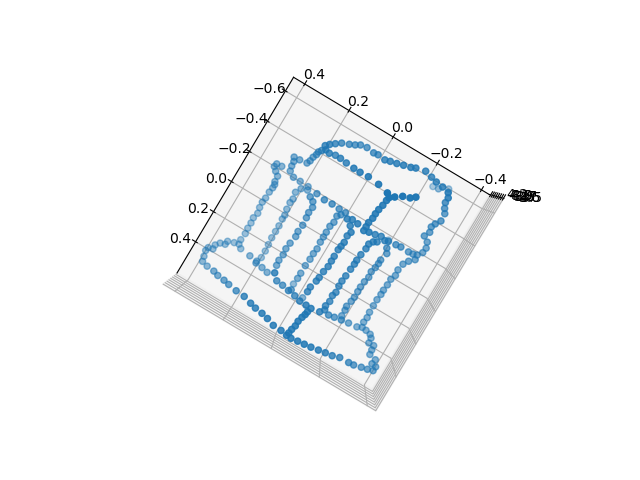
\includegraphics[width=\textwidth]{q4,2_1.png}
        \end{subfigure}
        \begin{subfigure}[b]{0.5\textwidth}
            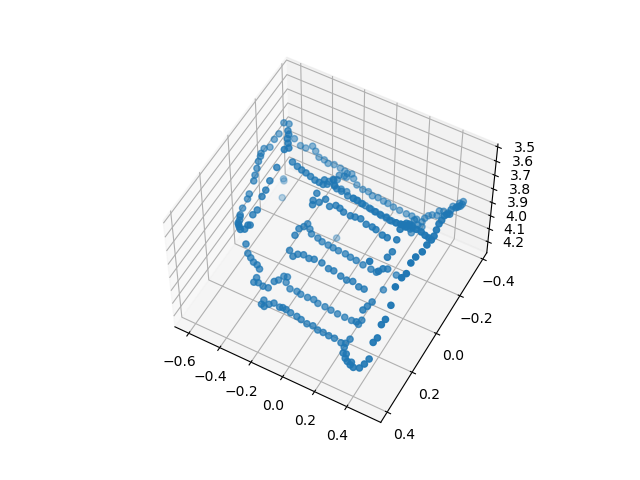
\includegraphics[width=\textwidth]{q4,2_2.png}
        \end{subfigure}
        \begin{subfigure}[b]{0.5\textwidth}
            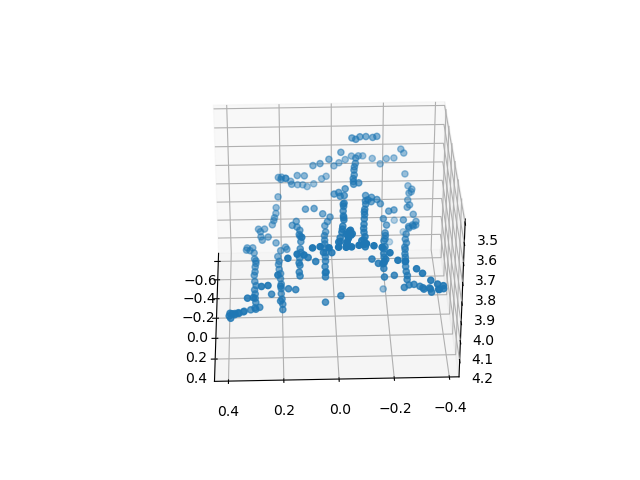
\includegraphics[width=\textwidth]{q4,2_3.png}
        \end{subfigure}
        \begin{subfigure}[b]{0.5\textwidth}
            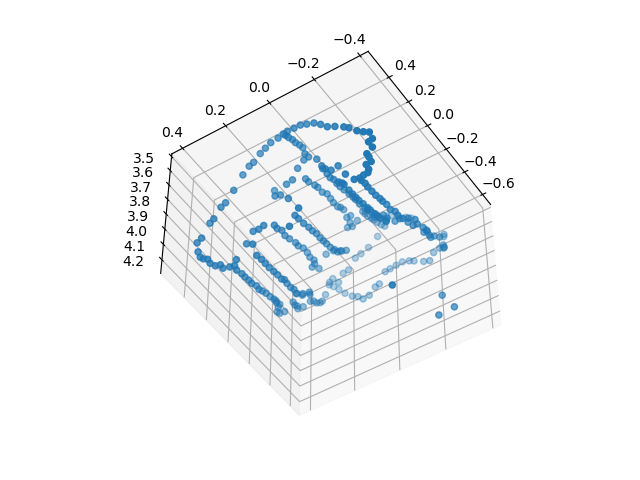
\includegraphics[width=\textwidth]{q4,2_4.png}
        \end{subfigure}
        \caption{3D Visualization}
    \end{figure}

    \section{Bundle Adjustment}
    \subsection*{Q5.1}

    Comparing the epipolar lines generated from the estimated fundamental matrix from \verb|eightpoint| and \verb|ransacF|, it is obvious that noisy correspondences will throw off the estimation greatly, and RANSAC can prevent that by selecting correct correspondences.
    \smallskip

    \begin{figure}[h]
        \begin{subfigure}[b]{0.5\textwidth}
            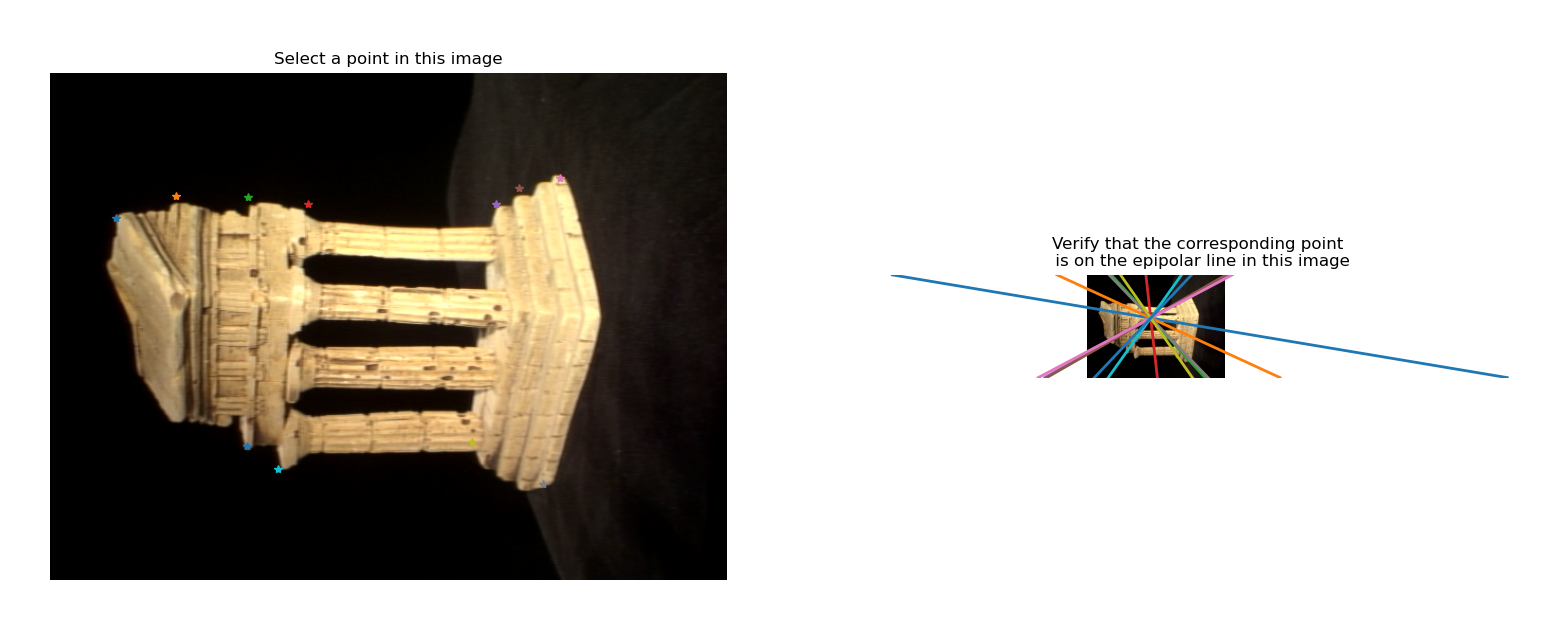
\includegraphics[width=\textwidth]{q5,1 eightpoint.png}
            \subcaption{}
        \end{subfigure}
        \begin{subfigure}[b]{0.5\textwidth}
            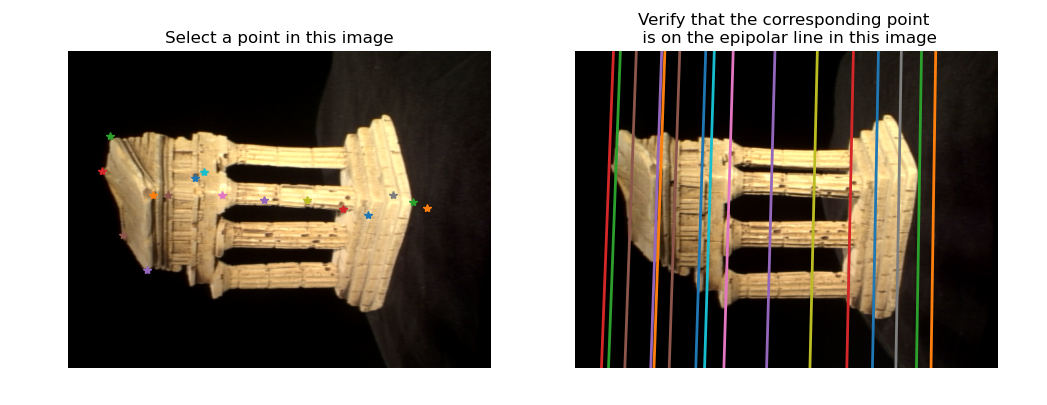
\includegraphics[width=\textwidth]{q5,1 ransac.png}
            \subcaption{}
        \end{subfigure}
        \caption{Comparison of fundamental matrix estimation performance by (a) \texttt{eightpoint} and (b) \texttt{ransacF}.}
    \end{figure}
    
    The error metric used is $\text{err}=|x_2^TFx_1|$, and a point is an inlier if $\text{err}$ is less than a certain threshold. Since refining the estimated fundamental matrix in \verb|sevenpoint| takes some time, \verb|multiprocessing| is used to speed up the process.

    \subsection*{Q5.3}

    The initial projection error is 104056.861470, and the projection error after bundle adjustment is 9.747948. Refer to the images for the 3D points.
    
    \smallskip
    Bundle adjustment was also run on \verb|templeCoords.npz|. Point correspondences from \verb|visualize.py| were optimized, and the reprojection error decreased from 203.3929 to 13.264073 after bundle adjustment.
    
    \begin{figure}[h]
        \begin{subfigure}[b]{0.5\textwidth}
            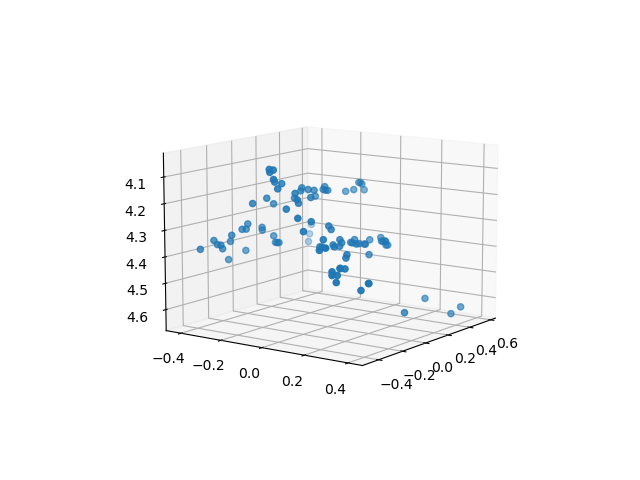
\includegraphics[width=\textwidth]{q5,3_init1.png}
            \subcaption{without bundle adjustment}
        \end{subfigure}
        \begin{subfigure}[b]{0.5\textwidth}
            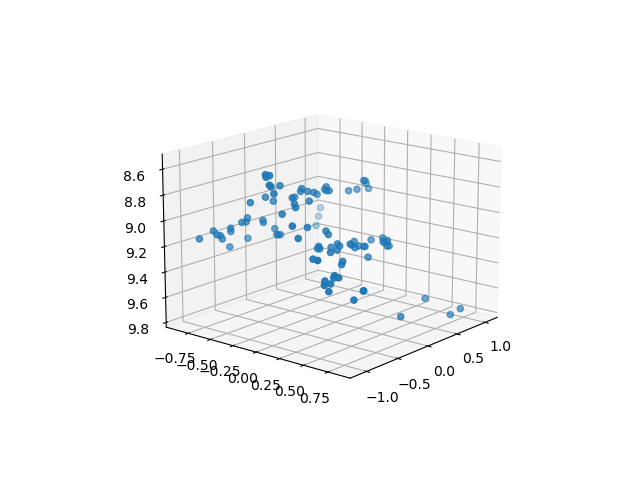
\includegraphics[width=\textwidth]{q5,3_opt1.png}
            \subcaption{with bundle adjustment}
        \end{subfigure}
        \caption{Comparison of noisy correspondences triangulation with and without bundle adjustment.}
    \end{figure}

    \begin{figure}[h]
        \begin{subfigure}[b]{0.5\textwidth}
            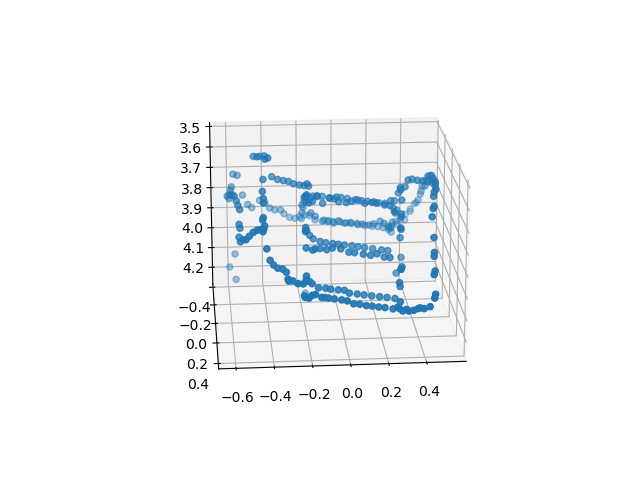
\includegraphics[width=\textwidth]{q5,3_init2.png}
            \subcaption{without bundle adjustment}
        \end{subfigure}
        \begin{subfigure}[b]{0.5\textwidth}
            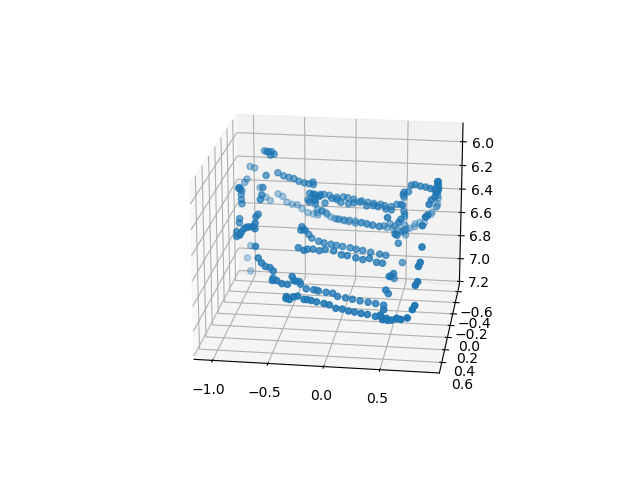
\includegraphics[width=\textwidth]{q5,3_opt2.png}
            \subcaption{with bundle adjustment}
        \end{subfigure}
        \caption{Comparison of \texttt{templeCoords.npz} triangulation with and without bundle adjustment.}
    \end{figure}
    
\end{document} % This is the end of the document